\documentclass[utf8, russian]{beamer}

\usepackage[utf8]{inputenc}
\usepackage[russian]{babel}
\usepackage{hyperref}
\usepackage{graphicx}
\usepackage{listings}
\usepackage{ucs}
\usepackage{clrscode}

\lstset{
    extendedchars=\true,
    inputencoding=utf8x
}

\usetheme{Warsaw}
\usecolortheme{lily}
\useoutertheme[subsection=false]{smoothbars}
\useinnertheme{circles}
\setbeamertemplate{footline}[page number]{}
\setbeamertemplate{navigation symbols}{}

\renewcommand{\figurename}{} 

\title{Архитектура ЭВМ}
\subtitle{Лекция 5. Стек и подпрограммы}
\author{к.ф.-м.н. Филонов Павел Владимирович \\ filonovpv@gmail.com}
\date{22 сентября 2013 г.}


\institute[МГТУ ГА] 
{
    Московский Государственный Технический Университет \\
    Гражданской Авиации
}
\begin{document}
    \frame{\titlepage}
    \begin{frame}{Сегодня поговорим о ...}
        \begin{itemize}
            \pause
            \item Что такое стек?
            \pause
            \item Процессор имеет им пользоваться
            \pause
            \item Зачем он нужен?
            \pause 
            \item Чем помогут подпрограммы?
            \pause
            \item А как они вообще работают?
            \pause
            \item Стековый фрейм --- вызрыв мозга или неизбежное зло?
            \pause
            \item Разные соглашения и передаче параметров
        \end{itemize}
    \end{frame}
    \section{Стек}
    \subsection{}
    \begin{frame}{Стек}

        {\bf Стек } ({\it англ.} Stack) --- структура данных, организованная по принципу LIFO (Last In --- First Out, последнием пришёл --- первым вышел)
    \begin{columns}
        \column{0.5\linewidth}
            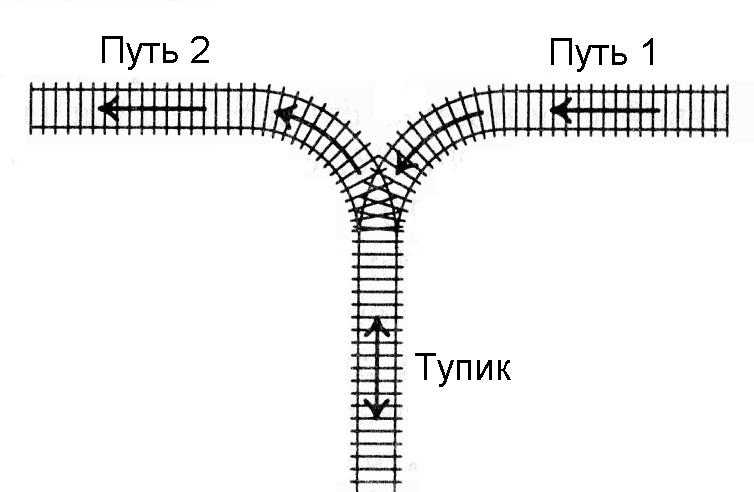
\includegraphics[width=\linewidth]{fig/stack_rails.jpg}
        \column{0.5\linewidth}
            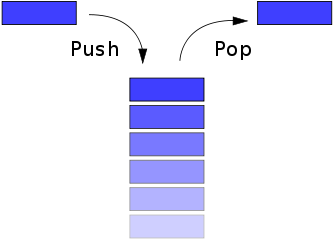
\includegraphics[width=\linewidth]{fig/stack.png}
    \end{columns}
    {\bf Push} --- положить элемент на вершину стека

    {\bf Pop} --- снять элемент с вершины стека
    \end{frame}
    \begin{frame}{Организация стека в архитектуре x86}
        \begin{columns}
        \column{0.5\linewidth}
        \begin{itemize}
            \item Секция стека располагается в старших адресах памяти. 
            \item Адрес вершины стека хранится в регисре ESP.
            \item Вершина стека растёт в сторону уменьшения адресов. 
        \end{itemize}
        \column{0.5\linewidth}
            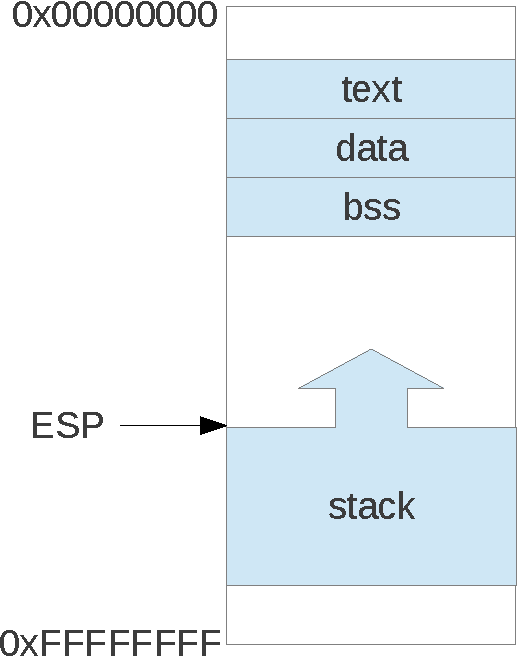
\includegraphics[width=\linewidth]{fig/segments.pdf}
        \end{columns}
    \end{frame}
    \begin{frame}{Команды работы со стеком}
        \begin{block}{Положить в стек}\small
            Команда {\bf push} помещает операнд на вершину стека и уменьшает ESP на размер операнда.
            \begin{itemize}
                \item push --- положить слово (2 байта) или двойное слово (4 байта)
                \item pushf (pushfd) --- положить в стека EFALGS (4 байта)
                \item pusha (pushad) --- положить в стек все 4-байтовые регистры (EAX, ECX, EDX, EBX, ESP, EBP, ESI, EDI) 
            \end{itemize}
        \end{block}
        \begin{block}{Взять со стека}\small
            Команда {\bf pop} извлекает с вершины стека данные, записывает их в операнд и увеличивает ESP на размер операнда
            \begin{itemize}
                \item pop --- извлечь слово (2 байта) или двойное слово (4 байта)
                \item popf (popfd) --- извлечь из стека EFALGS (4 байта)
                \item popa (popad) --- извлечь из стека все 4-байтовые регистры (EDI, ESI, EBP, EBX, EDX, ECX, EAX). Значение ESP пропускается             
            \end{itemize}
        \end{block}
    \end{frame}
    \begin{frame}{Пример (правильное скобочное выражение)}
        \begin{codebox}
            \Procname{Правильное скобочное выражение}
            \li \Comment возвращает True, либо False
            \li c $\leftarrow$ следующий символ
            \li \While не конец файла
            \li \Do \If c = '(' 
            \li     \Then push c
            \li     \Else \If c = ')'
            \li           \Then pop t
            \li                 \If t $\ne$ c
            \li                 \Then \Return False
                                \End
                          \End
                    \End
            \li     c $\leftarrow$ следующий символ
                \End
            \li \If стек не пуст
            \li \Then \Return False
            \li \Else \Return True
        \end{codebox}
    \end{frame}

    \section{Подпрограммы}
    \subsection{}
    \begin{frame}{Подпрограммы}
    \end{frame}
\end{document}